\documentclass{article}
 \usepackage[utf8]{inputenc}
 \usepackage{graphicx}
 \graphicspath{ {images/} }
 \begin{document}

 \title{ARTIFICIAL INTELLIGENCE EXAM}
 \author{Course Code: 1DL340}
 \date{Ref.  78889924-0-0-17689-35344-529-4356-0-1018081-144 }
 \maketitle

 This exam has  7  questions for a total of  21  marks. Grade boundaries are:

 \begin{center}
 3 -  10.5 

 4 -  14.0 

 5 -  17.5 

 \end{center}

 In exceptional circumstances these boundaries may be adjusted at the discretion of the examiner. This would be done on an exam-wide basis, NOT for individual students.

 You are permitted to make use of a calculator and language dictionary in this exam.
\clearpage
\section{A-Star}

Table~\ref{AStar_Edges} gives the edge values for a shortest path problem. Using these and the A* algorithm, find the shortest path from the start node to the goal node. Provide a valid heuristic and show all working. (4 marks)

\begin{table}[h!]
\caption{Edges}
\label{AStar_Edges}
\begin{center}
\begin{tabular}{ |c||c|c|c|c|c|c|c| } 
\hline
 & Start & A & B & C & D & E & Goal\\
\hline
Start & 0 & 5 & 7 & 0 & 3 & 0 & 0\\
A & 0 & 0 & 4 & 0 & 0 & 7 & 0\\
B & 0 & 0 & 0 & 4 & 6 & 4 & 0\\
C & 0 & 0 & 0 & 0 & 3 & 0 & 0\\
D & 0 & 0 & 0 & 0 & 0 & 2 & 0\\
E & 0 & 0 & 0 & 0 & 0 & 0 & 4\\
Goal & 0 & 0 & 0 & 0 & 0 & 0 & 0\\
\hline
\end{tabular}
\end{center}
\end{table}
\clearpage
\section{Hidden Markov Models: Viterbi Algorithm}

Tables~\ref{hmmvit1} to~\ref{hmmvit4} provide the transition matrix, emission matrix, initial state and a sequence of observations for a hidden Markov model. Use the Viterbi algorithm to calculate the most probable path and its probability.  TRUE=1, FALSE=0. Show all working. (3 marks)

\begin{table}[h!]
\caption{Transition Matrix}
\label{hmmvit1}
\begin{center}
\begin{tabular}{ |c||c|c| } 
\hline
 $S_{t-1}$ & $S_t$=0 & $S_t$=1\\
\hline
 0 & 0.3 & 0.7\\
 1 & 0.8 & 0.2\\
\hline
\end{tabular}
\end{center}
\end{table}
\begin{table}[h!]
\caption{Emission Matrix}
\label{hmmvit2}
\begin{center}
\begin{tabular}{ |c||c|c| } 
\hline
 $S$ & $E=0$ & $E=1$\\
\hline
 0 & 0.4 & 0.6\\
 1 & 0.8 & 0.2\\
\hline
\end{tabular}
\end{center}
\end{table}
\begin{table}[h!]
\caption{Initial State}
\label{hmmvit3}
\begin{center}
\begin{tabular}{ |c|c| } 
\hline
 $S=0$ & $S=1$\\
\hline
0.5 & 0.5\\
\hline
\end{tabular}
\end{center}
\end{table}
\begin{table}[h!]
\caption{Observations}
\label{hmmvit4}
\begin{center}
\begin{tabular}{ |c|c| } 
\hline
 Time=1 & Time=2\\
\hline
FALSE & FALSE\\
\hline
\end{tabular}
\end{center}
\end{table}
\clearpage
\section{Alpha-Beta Pruning}

Examine the game tree included in this exam. Note that the values in the nodes are node indices, not mini-max values. Perform alpha-beta pruning on this game tree.  You should show all working, where this means all alpha-beta values.  You can write these values on the diagram, or alternatively on a separate sheet of paper.  In both cases, provide a way of identifying the sequence of updates to alpha-beta values associated with nodes (we suggest you just cross out old values and write new values sequentially downwards).  If you write on a separate sheet of paper, use the node indices in the diagram as a way of identifying which node particular alpha-beta values are associated with.  Show where pruning occurs, by indicating which branches will not be evaluated.  Finally, provide the result (value at end state) of the game assuming optimal play. (3 marks)

\begin{figure}[h!]
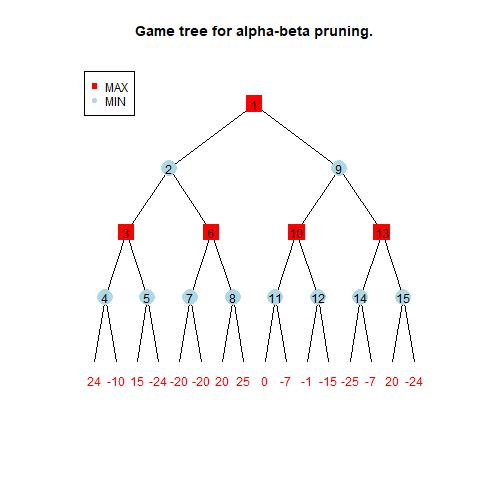
\includegraphics[width=\textwidth]{ab.jpg}
\end{figure}
\clearpage
\section{Scheduling}

Provide a complete resource constrained schedule for the actions found in Table~\ref{schActions}. (4 marks)
\begin{table}[h!]
\caption{Actions}
\label{schActions}
\begin{center}
\begin{tabular}{ |c|c|c|c|c|c| } 
\hline
 Index & Action & Duration & Uses & Consumes & After \\
\hline
1 & Start & 0 &   & 0 nails & NA\\
2 & Action 1 & 5 &  Saw & -1 nail & 1\\
3 & Action 2 & 30 &  Saw & 0 nails & 1\\
4 & Action 3 & 5 &  Saw & -1 nail & 1\\
5 & Action 4 & 35 &   & 1 nail & 3,4,2\\
6 & Action 5 & 5 &  Hammer & 0 nails & 2,3\\
7 & Action 6 & 30 &   & 1 nail & 6,5,2,4\\
8 & Action 7 & 50 &  Hammer & 0 nails & 2,5,7\\
9 & Finish & 0 &   & 0 nails & 8\\
\hline
\end{tabular}
\end{center}
\end{table}
\clearpage
\section{Multi-Armed Bandit Optimization}

Image we are testing click through rates on three different web layouts. At the current point, the Dirichlet (beta) distributions associated with each layout have the parameters in Table~\ref{MABO1}.\begin{table}[h!]
\caption{Dirichlet (Beta) Parameters for Layout}
\label{MABO1}
\begin{center}
\begin{tabular}{ |c|c|c| } 
\hline
 Layout & Parameter 1 & Parameter 2 \\
\hline
A &  9  &  5 \\
B &  8  &  5 \\
C &  9  &  2 \\
\hline
\end{tabular}
\end{center}
\end{table}

The first value is associated with not clicking through, the second clicking through.

A new person views the site. We generate samples from the distributions to determine which layout is used. These samples are given in Table~\ref{MABO2}.
\begin{table}[h!]
\caption{Samples from Layout Dirichlet (Beta) Distributions}
\label{MABO2}
\begin{center}
\begin{tabular}{ |c|c|c|c|c|c| } 
\hline
 Layout & Sample 1 & Sample 2 & Sample 3 & Sample 4 & Sample 5 \\
\hline
A &  0.25  &  0.44  &  0.61  &  0.43  &  0.4 \\
B &  0.5  &  0.38  &  0.34  &  0.46  &  0.38 \\
C &  0.08  &  0.06  &  0.12  &  0.29  &  0.22 \\
\hline
\end{tabular}
\end{center}
\end{table}


When shown the website with the chosen layout, the person makes a purchase ('clicks through'). Give the new parameters of the three distributions after this event. (2 Marks)
\clearpage
\section{ Iterated Deepening }

Explain iterated deepening. (2 marks)
\clearpage
\section{ Local Search }

Greedy Hill Climb suffers from the problem of local optima. Name and provide a brief explanation of three alternative local search strategies covered in this course that attempt to overcome or minimize this problem. (3 marks)

\end{document}
